\documentclass[compress,xcolor={dvipsnames}]{beamer}
\usepackage{fancyvrb,newverbs} % For customized verbatim
\usepackage{calligra} % A fancy text for ending `Thank you'
\usepackage[T1]{fontenc}
\usefonttheme[onlymath]{serif}

\author{Zihang Wang}
\title{Phase Field Tutorial}
\subtitle{Mathematics 2: Numerical Methods with Python Implementation}
\institute{Central South University}

\AtBeginSubsection[]
{
	\begin{frame}
		\tableofcontents[sectionstyle=show/shaded,subsectionstyle=show/shaded/hide,subsubsectionstyle=show/shaded/hide]
	\end{frame}
}
\usetheme{Berlin}

\setbeamertemplate{footline} {
    \begin{beamercolorbox}[ht=2.5ex,dp=1.125ex,
      leftskip=.3cm,rightskip=.3cm plus1fil]{title in head/foot}
      {\usebeamerfont{institute in head/foot}\usebeamercolor[fg]{institute in head/foot}\insertshortinstitute}
      \hfill
      {\centering\usebeamerfont{title in head/foot}\insertshortsubtitle}
      \hfill
      {\usebeamerfont{frame number}\usebeamercolor[fg]{frame number}\insertframenumber~/~\inserttotalframenumber}
    \end{beamercolorbox}
    \begin{beamercolorbox}[colsep=1.5pt]{lower separation line foot}
    \end{beamercolorbox}
}

% ---------------------------------------------------------------------------
\definecolor{cverbbg}{gray}{0.93}

\newenvironment{cverbatim}
 {\SaveVerbatim{cverb}}
 {\endSaveVerbatim
  \flushleft\fboxrule=0pt\fboxsep=.5em
  \colorbox{cverbbg}{\BUseVerbatim{cverb}}%
  \endflushleft
}
\newenvironment{lcverbatim}
 {\SaveVerbatim{cverb}}
 {\endSaveVerbatim
  \flushleft\fboxrule=0pt\fboxsep=.5em
  \colorbox{cverbbg}{%
    \makebox[\dimexpr\linewidth-2\fboxsep][l]{\BUseVerbatim{cverb}}%
  }
  \endflushleft
}
\newverbcommand{\cverb}
  {\setbox\verbbox\hbox\bgroup}
  {\egroup\colorbox{cverbbg}{\box\verbbox}}

\setlength{\parindent}{2em}

\newcommand{\bhref}[2]{
    \href{#1}{\color{blue}{#2}}
}
% ---------------------------------------------------------------------------

\begin{document}
\begin{frame}
    \titlepage
    \begin{figure}[!h]
        \centering
        
\includegraphics[width=0.18\linewidth]{pic/csulogo.jpg}
        
\includegraphics[width=0.25\linewidth]{pic/MInDes_Icon.jpg}
    \end{figure}
\end{frame}

\begin{frame}
    \tableofcontents[currentsection, hideothersubsections, sectionstyle=show/show]
\end{frame}

% ---------------------------------------------------------------------------
\section{Review \& Intro}
\begin{frame}
    \frametitle{Quick Review}
    What have we got in the last tutorial?

    \begin{itemize}
        \item Intro to PF
        \item Taylor Formula
        \item Extrema with Constraint
        \item Variational Derivative
        \item Vector Calculus
    \end{itemize}

    Great, let's move on.
\end{frame}

\begin{frame}
    \frametitle{Numerical Method}
    By now, you should have acquired the basic knowledge about phase field method. But how to carry out a simulation?
    \bigbreak
    \pause
    The answer is: \emph{Numerical analysis}, or \emph{numerical methods}. That means breaking the mathematical problem into pieces and converting to computer programming
    problems, then using programming to solve them.
    \bigbreak
    \pause
    So, in today's tutorial, we are going to cover some numerical methods, together with how to implement them with a programming language.
    Here we choose Python to implement these algorithms
    \footnote<.(1)->{While, next tutorial will focusing on C++, a faster but more complex programming language}.
    Don't worry, we will also cover some points about python, start from scratch.
\end{frame}

% ---------------------------------------------------------------------------
\section{Preliminary}
\subsection{To achieve our goal \dots}
\begin{frame}
    \frametitle{What Questions Are We Facing?}
    As you can see, numerical analysis is a general concept, and for a particular problem, there should be a particular method, or say, algorithm, to solve it.
    And to find the proper methods to solve our questions, we should analysis the questions we are facing.

    Let's look back at the two governing questions we mentioned before:
    \[
        \frac{\partial c_i}{\partial t} = \nabla \cdot M_{ij} \nabla \frac{\delta F}{\delta c_j \left( r,t \right)} \tag{Cahn-Hilliard}
    \]
    \[
        \frac{\partial \eta_p}{\partial t} = -L_{pq}\frac{\delta F}{\delta\eta_q\left( r,t \right)} \tag{Allen-Cahn}
    \]
    So, the main question is, how to utilise these equations to evolute the field parameter as we want?
\end{frame}

\begin{frame}
    \frametitle{Break Down the Questions}
    By analysising these two equations (don't forget the exercises in the last tutorial), the following questions should be solved:
    \pause
    \begin{itemize}
        \item How to solve \emph{ordinary differential equations} and \emph{partial differential equations} (usually refered as \emph{ODE} and \emph{PDE})?
        \item How to \emph{Integrate}?
        \item How to deal with \(\nabla\)? (that is, how to \emph{taking derivative})
        \item How to (, if you have seen more about vector analysis,) deal with \(\nabla^2\)(\emph{laplacian}, sometimes denoted as \(\Delta\))?
    \end{itemize}
    \pause
    With these sub-questions solved, and a little bit of code, we should be able to, finally, start a (simple) simulation by ourselves, independently.
\end{frame}

\begin{frame}
    \frametitle{How Numerical Methods Work?}
    One of the most obvious features of numerical methods is it use `discrete' to replace `continuous'. For example, taking derivative
    can be approximated by small value interval divided by small variable interval, and integrate can be approximated by sum of small variable interval
    times its corresponding mean value. Or, to make it clearer, in analytical method, you taking limit to achieve `continuous', while in
    numerical method, you taking small interval to mimic limit.
    \bigbreak
    \pause
    By now you may have gotten idea of how to solve the sub-questions we mentioned above. If so, all you need is a great tool to check your idea.
    Here it comes: Python.
\end{frame}

\subsection{Welcome to Python!}
\begin{frame}
    \frametitle{What's Python?}
    Python is a kind of snake, and in the mean time, one of the most popular programming language in the world. Easy to learn, friendly grammar, and most important,
    its large community, together with hundreds and thousands of great tutorials are Python's outstanding features.
    \bigbreak
    \pause
    Let's start from the scratch, that is: download the interpreter first\footnote<.(1)->{What is interpreter? While, loosely speaking, it's a program that interprets
        code to computer and let computer to execute it. It differs from compiler (used by C/C++) that interpreter translates and executes code line by line, while compiler
        must compile the code to binary file (usually, on Windows, an \emph{exe} file) and then execute it}.
\end{frame}

\begin{frame}
    \frametitle{Let's start with Python}
    Let's suppose your operating system is Windows\footnote{For users of *nix users, things are easier that just install it with the package manager you have (or like)}.
    Head to \bhref{https://www.python.org/downloads/}{{Python's download page}}, hit the `Download' button,
    waiting for the downloading to complete, then you will get the installer. Install it, but remember,
    \bigbreak
    \pause
    \centerline{\large TOGGLE ADD TO THE PATH CHECKBOX!}
    \begin{figure}
        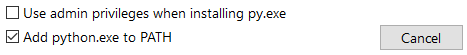
\includegraphics[width=0.7\linewidth]{pic/PythonInstall.png}
    \end{figure}
    \pause
    Then you can just accept the default settings, and after installing, you are ready for coding with Python
    \footnote<.(1)->{Or, you can using \emph{Microsoft Store} to download Python interpreter, or using package manager to achieve this.}.
\end{frame}

\begin{frame}[fragile]
    \frametitle{Check your installation}
    You must can't wait coding with Python, but before that, please check wheather you have installed your interpreter successfully:
    \begin{enumerate}
        \item Open a shell (cmd or powershell, you can use \cverb|win + R| to open `run' and input \cverb|cmd| (if you prefer powershell, \cverb|powershell|))
        \item Input {\cverb|python --version|} and hit {\cverb|Enter|}.
        \item If you installed successfully, you will get the version information about python.
        \item While, if you get something like `\emph{XXXX is not reconised as xxx}',
              that error message indicates that you might forget to \emph{add python.exe to PATH}. Re-install or add to PATH manually.
    \end{enumerate}
\end{frame}

\begin{frame}[fragile]
    \frametitle{Begin your first Python code}
    Now, please create a text file, modify its extension name
    (if you didn't see anything with \cverb|.txt|, open extension name in file explorer options) to \cverb|py|, and open it. Then write the following code:
    \begin{lcverbatim}
        print("Hello Python World!")
    \end{lcverbatim}
    Save it, which is your first python script. Then open the shell you like, call python interpreter with your script's path as argument:
    \begin{lcverbatim}
        python C:\path\to\your\python\script
    \end{lcverbatim}
    \emph{Remember to replace the} \cverb|C:\path\to\your\python\script| \emph{to your script's path.}
    You should see `Hello Python World' was printed in your shell.
\end{frame}

\begin{frame}
    \frametitle{Edit in Plain Text?}
    Congrats, you should have made your first step in Python programming. But wait, shall one edit the python script in plain text editor?
    The answer is: no, of course not. What you need is a modern editor to handle it.

    Here I recommend Visual Studio Code with Python
    extension, and run or edit Python with Jupyter Notebook. You can go to \bhref{https://github.com/A-moment096/Python-with-VSCode}{my Github repository}
    to download the instruction about how to set up a Python environment with VS Code. There will also be a \bhref{}{repository} contains today's code and other resources.
    Comments and suggestions about these documents are welcomed.

    Of course, developing large-scaled Python program usually use \emph{Integrated Development Environment}, \emph{IDE}. The most famous one might be
    \bhref{https://www.jetbrains.com/pycharm/}{PyCharm} by \emph{JetBrains}. Try it if you want.

\end{frame}

\begin{frame}
    \frametitle{A Python Tutorial?}
    By far, we are all talking about Python. One might complain that: `Is this a Python tutorial?'
    \bigbreak
    \pause
    We will pause for a while. For thouse who are completely new to Python, the following part is focusing on algorithm, and we will turn to Python 
    in the time we need to implement these algorithms. If you need aids with Python language, there are so many awesome tutorials about Python, 
    from beginer to proficient. If you'd like to learn more about Python, please head for \hyperlink{fm_resources}{\color{YellowGreen}these} resources.
    \bigbreak
    \pause
    Now, we are prepared for Python programming, meaning that we are
    ready to write Python scripts and implement our algorithms with Python (although you might be not familiar with Python yet).
\end{frame}
% ---------------------------------------------------------------------------
\section{Numerical Methods}
\subsection{ODE\&PDE}
\begin{frame}
    \frametitle{What are ODE and PDE?}
    ODE and PDE are equations that the solutions are a function(precisely, a family of functions). As their name indicates, ODE contains
    total derivative, while PDE contains partial derivative. Let's give the definitions for these two concepts:
    \begin{block}{Ordinary (Partial) Differential Equation}
        Given \(F\), a function of \(x\), \(y\), and derivatives of \(y\), the equation of the form
        \[F(x,y,y',\dots,y^{(n)}) = 0\]
        is called an ordinary differential equation (partial differential equation, if derivatives stands for partial derivative).
        Then, a n-times differentiable function \(u\) satisfies this equation is thus a solution to this ODE (or PDE).
    \end{block}
\end{frame}

\begin{frame}
    \frametitle{Analytical Solutions vs. Numerical Solutions}
    You might want to get an analytical solution of a ODE or PDE. Usually it's possible only in homework, and impractical when
    facing a little bit more complicated equation.
    \bigbreak
    Analytical solution provides to some extent perfect solution to a equation, while
    in practice, especially in physical or material context, analytical result is `way more precise' than actual needs, and numerical
    result can provide a balance between less time consuming with lower precision. And sometimes, numerical method is the only way to
    solve a over-complicated differential equation.
    \bigbreak
    \pause
    So, let's head for the numerical method of solving differential equations. Here we are going to introduce
    \emph{forward (explicit) Euler method} and \emph{backward (implicit) Euler method}, included in \emph{finite difference method (FDM)}.
\end{frame}

\begin{frame}
    \frametitle{Difference Quotient}
    Consider a function's Taylor expansion at point (denote the interval as \(\Delta x\)):
    \[
        f(x+\Delta x) = f(x) + \frac{f'(x)}{1!}\Delta x+\dots+\frac{f^{n}(x)}{n!}\left(\Delta x\right)^n+r_n(x;x+\Delta x),
    \]
    Now, we want to get approximation of first order differentials, \(\tilde{f}'\). To achieve that, take the higher terms to be reminder and eliminate the
    reminder, and you will get:
    \[ \tilde{f}'(x) = \frac{f(x+\Delta x) - f(x)}{\Delta x}  \]
    That's so called \emph{first order difference quotient}. If you need higher order one, you can calculate it recursively, by taking
    \(n\)th step result as \(n+1\)th step's input.
    \bigbreak
    \pause
    Now it's time to try a simple example:
\end{frame}

\begin{frame}
    \frametitle{Euler Method from Simple Example}
    Consider a simple differential equation as follows:
    \[\frac{\mathrm{d} y}{\mathrm{d} t} = f(t,y),\]
    and suppose you have already know the start point \(\left( 0, u(0) \right)\) of the graph of the solution function \(u\)
    \footnote{With initial condition, this problem belongs to initial value problems (IVP).}.
    By subsituting derivative with difference quotient, and labelling the value of the solution function
    \(u\) at each divided points as \(u_1 = u(0+\Delta t)\), \(u_2 = u(0+2\Delta t)\),\dots
    \bigbreak
    \pause
    Now this differential equation can be written as:
    \[\frac{u_n - u_{n-1}}{\Delta t} = f(t,\underline{u}).\]
\end{frame}

\begin{frame}
    \frametitle{Explicit \& Implicit Euler Method}
    Here is a underlined notation, \(\underline{u}\). That should be the value of \(u\) at the point \(t\). What should it be?
    \bigbreak
    \pause
    If you choose \(u_{n-1}\) as  \(\underline{u}\), then you get \emph{forward Euler method}. Just multiply \(\Delta t\) to the RHS,
    then move \(u_{n-1}\) to the RHS, you get the formula to derive the value of \(u\) from \(t = 0\) to wherever you want. Quite easy, right?
    \bigbreak
    \pause
    If you choose \(u_n\) as \(\underline{u}\), then you get \emph{backward Euler method}. You must have seen that in this case, you can't
    directly solve \(u_n\) instantly. That's why it is also refered as \emph{implicit Euler method}, and another one method also named
    \emph{explicit Euler method}.
    \pause
    \bigbreak
    Well, what if choosing other values?
\end{frame}

\begin{frame}
    \frametitle{Do it with Python!}
    Believing this is the time to implement this algorithm with Python, please try it yourself.
    \bigbreak
    You will get hints from the given resources.
\end{frame}

\subsection{Integrate}
\begin{frame}
    \frametitle{Sum It Like Riemann, in Python}
    You have already know how to approximate a function's derivative. Just imagine how to get
    approximation of integral.
    \bigbreak
    \pause
    So remind yourself with Riemann integral's definition. Dividing function's domain into small pieces, then
    times them with corresponding function value, and sum them up. If you continue to take limit of the domain pieces,
    you get Riemann integral\footnote<.(1)->{Actually, Riemann integral's definition is more general that, the domain's
    division is arbitrary, any division should give the same results, and so on. We don't cover these here}. 
    But if you stop here, you get a approximation of (Riemann) integral.
    \bigbreak

\end{frame}
\begin{frame}
    \frametitle{OOP, and other algorithm}
    Integrate single variable functions using plain Riemann or Darboux summation, should be somehow a simple thing. So we'll
    try to integrate double variable functions. This brings a problem: How can I define a double variable function? Here we introduce:
    \emph{OOP}, \emph{Object Oriented Programming}.
    \bigbreak
    \pause
    OOP aimings at gathering several related data together, with functions describing how these data are processed and cooperate with each other, inner or outer.
    A collection of such things is called \emph{object}, with data called \emph{property} and function called \emph{method}.
    \bigbreak
    \pause
    Aside for the plain sum, there are indeed some better algotithms to do numerical integral. While, talk is cheap. Let's head for the code.

\end{frame}

\subsection{\texorpdfstring{$\nabla$}{nabla} \& \texorpdfstring{$\nabla^2$}{nabla\^{}2}}
\begin{frame}
    \frametitle{Nothing but Derivative}
    The title reveals it all. What we need is just extend the differential from one dimension to higher dimension. 
    \bigbreak
    \pause
    But it \emph{is} the higher dimension matters. We are going to, again, use OOP to handle this problem.
    \bigbreak
    \pause

    We are going to implement the \(\nabla\), gradient and laplacian with Python, and utilise the feature of OOP.
\end{frame}
% ---------------------------------------------------------------------------
\section{Summary}
\begin{frame}
    \frametitle{Sum it up}
    What did we get by now?
    \begin{itemize}
        \item Numerical methods for solving differential equations, integrates, gradient and laplacian.
        \item Basic knowledge about programming.
        \item Some Python skill enabling one to do many things.
    \end{itemize}

\end{frame}
\begin{frame}[label=fm_resources]
    \frametitle{Resources}
    Here's a list of recommended resources.
    \begin{itemize}
        \item \bhref{https://ocw.mit.edu/ans7870/2/2.086/F14/MIT2_086S13_Textbook.pdf}{Math, Numerics, \& Programming (for Mechanical Engineers)}
        introduces a lot of practical numerical methods together with some programming implementation.
        \item \bhref{https://github.com/A-moment096/Python-with-VSCode}{My Github repository} about Python developing environment set up with VS Code
        and Jupyter notebook.
        \item \bhref{https://www.runoob.com/python3/python3-tutorial.html}{Runoob} provides good introduction and basic usage of Python.
        \item \bhref{https://www.python.org/doc/}{Python documentation set} for who interested in Python with details.
        \item  \emph{Python Crash Course} is a good Python book for beginers. Its resources collection is in \bhref{https://github.com/ehmatthes/pcc_3e}{Github}.
        \item If you meet any question with any package/module, please refer to its documentation site.
    \end{itemize}
\end{frame}

\end{document}
